\documentclass[tikz,border=7pt]{standalone}
\usepackage{amsmath}
\begin{document}
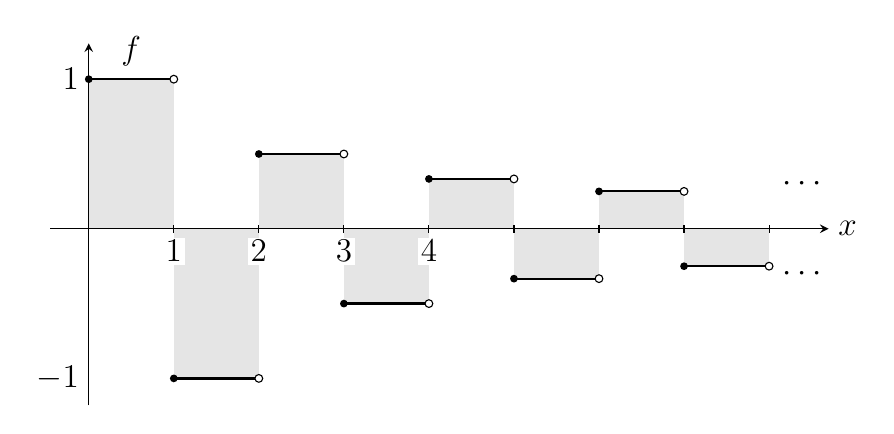
\begin{tikzpicture}[x=1.08cm,y=1.9cm,>=stealth,font=\large]
  \foreach \n in {0,...,3} {
    \pgfmathsetmacro{\height}{1/(\n+1)}
    \fill[black!10] ({2*\n},0) rectangle ({2*\n+1},\height);
    \fill[black!10] ({2*\n+1},0) rectangle ({2*\n+2},-\height);
    \draw[thick] ({2*\n},\height) -- ({2*\n+1},\height);
    \draw[thick] ({2*\n+1},-\height) -- ({2*\n+2},-\height);
    \fill ({2*\n},\height) circle (1.4pt)
          ({2*\n+1},-\height) circle (1.4pt);
    \draw[fill=white] ({2*\n+1},\height) circle (1.4pt)
                     ({2*\n+2},-\height) circle (1.4pt);
  }
  \draw[->,thin] (-0.45,0) -- (8.7,0) node[right] {$x$};
  \draw[->,thin] (0,-1.18) -- (0,1.24);
  \foreach \x in {1,...,8} {
    \draw[thin] (\x,-0.025) -- (\x,0.025);
  }
  \foreach \x in {1,...,4} {
    \node[below=3pt,fill=white,inner sep=1pt] at (\x,0) {$\x$};
  }
  \node[left] at (0,1) {$1$};
  \node[left] at (0,-1) {$-1$};
  \node[above] at (0.5,1.02) {$f$};
  \node at (8.42,0.3) {$\cdots$};
  \node at (8.42,-0.3) {$\cdots$};
\end{tikzpicture}
\end{document}
